\documentclass[aspectratio=169]{beamer}

% Shared Beamer settings for Applied Machine Learning lectures (UPES).
% Keep this file free of \documentclass to allow reuse via \input.

% Allow lecture sources to use shared theme/assets without copying them into each lecture folder.
% NOTE: These paths are relative to `Unit-xx/Lecture-yy/latex/` (and `Lab/Experiment-xx/latex/`).
\makeatletter
\def\input@path{{../../../_shared/}{../../../_shared/UPES-Beamer-Theme/}}
\makeatother

\usetheme{UPES}
\setbeamertemplate{navigation symbols}{}

\usepackage{amsmath}
\usepackage{amssymb}
\usepackage{booktabs}
\usepackage{graphicx}
\usepackage{hyperref}
\usepackage{xcolor}
\usepackage{listings}

% Code listings (Python-oriented for this subject).
\lstset{
  language=Python,
  basicstyle=\ttfamily\small,
  keywordstyle=\color{blue},
  commentstyle=\color{gray},
  stringstyle=\color{teal},
  showstringspaces=false,
  columns=fullflexible,
  breaklines=true
}

\usepackage{tikz}
\usetikzlibrary{arrows.meta,positioning,shapes.geometric,calc,fit,backgrounds}

% Per-slide source line (references shown on the slide itself).
\newcommand{\slidesources}[1]{%
  \vfill
  {\tiny\color{gray}\raggedright\sloppy\parbox{\linewidth}{Sources: #1}\par}%
}

% Unit-wise source strings for this subject (used by slides/notes).
% Path is relative to the lecture `latex/` folder (the compilation CWD).
% Source strings for Applied Machine Learning (CSAI2017P) — used by slides + notes.
% Prescribed texts and reference books are taken from the course syllabus.
% Support texts are the author-hosted open-access editions:
%   statlearning.com            (ISL with Python)
%   probml.github.io/pml-book   (Murphy, Probabilistic Machine Learning)
%   d2l.ai                      (Dive into Deep Learning)
%   mml-book.github.io          (Mathematics for Machine Learning)

\newcommand{\AMLRepoURL}{https://github.com/tali7c/Applied-Machine-Learning}

% --- prescribed -------------------------------------------------------------
\newcommand{\AMLPrescribed}{%
M\"uller and Guido, \textit{Introduction to Machine Learning with Python}, O'Reilly, 2016.;%
Bishop, \textit{Pattern Recognition and Machine Learning}, Springer, 2006.;%
Murphy, \textit{Machine Learning: A Probabilistic Perspective}, MIT Press, 2012.;%
Han, Kamber and Pei, \textit{Data Mining: Concepts and Techniques} (3e), Morgan Kaufmann, 2012.%
}

% --- unit-wise ---------------------------------------------------------------
\newcommand{\AMLUnitISources}{%
M\"uller and Guido, \textit{Introduction to Machine Learning with Python}, Ch. 1.;%
Bishop, \textit{Pattern Recognition and Machine Learning}, Ch. 1.;%
Murphy, \textit{Probabilistic Machine Learning: An Introduction}, MIT Press, 2022, Ch. 1.;%
Mitchell, \textit{Machine Learning}, McGraw Hill, 1997, Ch. 1.;%
Scikit-learn documentation, accessed 2026-08-04.%
}

\newcommand{\AMLUnitIISources}{%
Bishop, \textit{Pattern Recognition and Machine Learning}, \S1.5, \S4.3, \S7.1.;%
Zhang, Lipton, Li and Smola, \textit{Dive into Deep Learning}, \S3.4.;%
Shalev-Shwartz and Ben-David, \textit{Understanding Machine Learning}, Ch. 15.;%
Murphy, \textit{Probabilistic Machine Learning: An Introduction}, Ch. 5.%
}

\newcommand{\AMLUnitIIISources}{%
Zhang, Lipton, Li and Smola, \textit{Dive into Deep Learning}, Ch. 12 (Optimization Algorithms).;%
Deisenroth, Faisal and Ong, \textit{Mathematics for Machine Learning}, Ch. 7.;%
Kingma and Ba, ``Adam: A Method for Stochastic Optimization,'' ICLR 2015.;%
Ruder, ``An overview of gradient descent optimization algorithms,'' arXiv:1609.04747, 2016.%
}

\newcommand{\AMLUnitIVSources}{%
Han, Kamber and Pei, \textit{Data Mining: Concepts and Techniques} (3e), Ch. 3.;%
M\"uller and Guido, \textit{Introduction to Machine Learning with Python}, Ch. 3--4.;%
James, Witten, Hastie, Tibshirani and Taylor, \textit{An Introduction to Statistical Learning with Python}, Ch. 5--6, 12.;%
Scikit-learn documentation (preprocessing, model selection), accessed 2026-08-04.%
}

\newcommand{\AMLUnitVSources}{%
James et al., \textit{An Introduction to Statistical Learning with Python}, Ch. 3--6.;%
Bishop, \textit{Pattern Recognition and Machine Learning}, Ch. 3.;%
Deisenroth, Faisal and Ong, \textit{Mathematics for Machine Learning}, Ch. 9.;%
M\"uller and Guido, \textit{Introduction to Machine Learning with Python}, \S2.3.%
}

\newcommand{\AMLUnitVISources}{%
Han, Kamber and Pei, \textit{Data Mining: Concepts and Techniques} (3e), Ch. 8--9.;%
James et al., \textit{An Introduction to Statistical Learning with Python}, Ch. 8--9.;%
Bishop, \textit{Pattern Recognition and Machine Learning}, Ch. 4--5, 7, 14.;%
Zhang et al., \textit{Dive into Deep Learning}, Ch. 5.%
}

\newcommand{\AMLUnitVIISources}{%
Han, Kamber and Pei, \textit{Data Mining: Concepts and Techniques} (3e), Ch. 10.;%
James et al., \textit{An Introduction to Statistical Learning with Python}, Ch. 12.;%
M\"uller and Guido, \textit{Introduction to Machine Learning with Python}, \S3.5.;%
Ester, Kriegel, Sander and Xu, ``A density-based algorithm for discovering clusters (DBSCAN),'' KDD 1996.%
}

\newcommand{\AMLLabSources}{%
M\"uller and Guido, \textit{Introduction to Machine Learning with Python}, companion notebooks.;%
McKinney, \textit{Python for Data Analysis} (3e), O'Reilly, 2022.;%
Scikit-learn user guide, accessed 2026-08-04.;%
Matplotlib and Seaborn documentation, accessed 2026-08-04.%
}



\graphicspath{{../figures/}{../images/}{../../../_shared/}{../../../_shared/UPES-Beamer-Theme/}}

\title[Applied Machine Learning]{Applied Machine Learning}
\subtitle{Unit 07 -- Lecture 21: Similarity Measures and Data Types in
Clustering}
\author{Tofik Ali}
\institute{School of Computer Science, UPES Dehradun}
\date{Autumn 2026}

% ---- a compact "output" block so code and its result sit together ----------
\lstdefinestyle{outblk}{
  basicstyle=\ttfamily\scriptsize\color{black!75},
  backgroundcolor=\color{black!5}, frame=leftline, framerule=2pt,
  rulecolor=\color{black!30}, breaklines=true, columns=fullflexible,
  keepspaces=true,   % several outputs below are aligned tables
  language={},       % printed output is not Python: do not syntax-highlight it
  xleftmargin=4pt, aboveskip=1pt, belowskip=1pt, literate={-}{{-}}1}
\lstnewenvironment{outblk}{\lstset{style=outblk}}{}

\begin{document}

\UPESCoverFrame
\setcounter{framenumber}{0}

\begin{frame}[shrink=4]
  \titlepage
  \begin{center}
    \footnotesize Every clustering algorithm takes a distance as input\\[0.25em]
    \footnotesize Topic focus: \textbf{get the distance right before you run
    anything}\\[0.25em]
    \footnotesize Repository: \texttt{\AMLRepoURL}
  \end{center}
  \slidesources{\AMLUnitVIISources}
\end{frame}

\begin{frame}{Quick Links}
  \centering
  \hyperlink{sec:axioms}{\beamerbutton{What a distance must be}}\hspace{0.4em}
  \hyperlink{sec:mink}{\beamerbutton{Minkowski family}}\hspace{0.4em}
  \hyperlink{sec:cos}{\beamerbutton{Cosine vs Euclidean}}\hspace{0.4em}
  \hyperlink{sec:bin}{\beamerbutton{Binary attributes}}\\[0.6em]
  \hyperlink{sec:nomord}{\beamerbutton{Nominal and ordinal}}\hspace{0.4em}
  \hyperlink{sec:mixed}{\beamerbutton{Mixed types}}\hspace{0.4em}
  \hyperlink{sec:std}{\beamerbutton{Standardisation}}\hspace{0.4em}
  \hyperlink{sec:cent}{\beamerbutton{Centroids and linkage}}\hspace{0.4em}
  \hyperlink{sec:summary}{\beamerbutton{Summary}}
\end{frame}

\begin{frame}{Agenda}
  \tableofcontents
\end{frame}

\begin{frame}[shrink=14]{How this lecture works}
  \begin{columns}[T]
    \begin{column}{0.48\textwidth}
      \begin{block}{Every idea appears twice}
        \begin{enumerate}
          \item \textbf{By hand} --- two points, three patients, four
            applicants, six points on a page. Small enough to check with a
            pen.
          \item \textbf{In code} --- the same arithmetic again inside
            \texttt{scipy} and \texttt{scikit-learn}, so you can see the
            library is doing exactly this and nothing magic.
        \end{enumerate}
      \end{block}
    \end{column}
    \begin{column}{0.48\textwidth}
      \begin{alertblock}{Commit before you look}
        Five slides ask you to predict a number, or a winner, before it is
        revealed. Write your guess down. Being wrong on paper is how the
        idea sticks.
      \end{alertblock}
    \end{column}
  \end{columns}
  \vspace{0.4em}
  \begin{center}
    \small This is the most \textbf{numerical} lecture in the unit. The
    binary contingency table and the mixed-type table are the two
    calculations you should be able to reproduce with a pen, and both are
    examinable.
  \end{center}
\end{frame}

\begin{frame}{One seed, and three places it is used}
  \begin{columns}[T]
    \begin{column}{0.48\textwidth}
      \begin{block}{The data}
        \small Bundled \texttt{load\_wine}, \texttt{load\_iris},
        \texttt{load\_breast\_cancer}, and small tables typed out in the
        code. Nothing is downloaded and nothing is generated.
      \end{block}
    \end{column}
    \begin{column}{0.48\textwidth}
      \begin{block}{The randomness}
        \small One seed for the whole lecture:
        \texttt{np.random.default\_rng(0)}, also \texttt{random\_state=0}.
        The $200$ axiom points, the $400$ ordering pairs, one
        \texttt{KMeans}. Every listing shows it.
      \end{block}
    \end{column}
  \end{columns}
  \vspace{0.5em}
  \begin{exampleblock}{Why this matters to you}
    \centering\small
    Every number in this deck is printed by one script. Run the code as
    written and you get the same numbers --- which is the only reason to
    believe a number on a slide.
  \end{exampleblock}
\end{frame}

\begin{frame}[shrink=14]{Where we are}
  \begin{columns}[T]
    \begin{column}{0.47\textwidth}
      \begin{block}{The previous lecture defined the problem}
        Clustering groups objects so that objects in the same group are
        \emph{similar} and objects in different groups are not. No labels,
        no supervision, no test set.
      \end{block}
      \begin{block}{It left one word undefined}
        \textbf{Similar.} Every algorithm in this unit --- hierarchical,
        $k$-means, $k$-medoids, DBSCAN --- takes a distance as its input and
        is only as good as that distance.
      \end{block}
    \end{column}
    \begin{column}{0.49\textwidth}
      \begin{exampleblock}{Today's one question}
        Given two rows of a table, how far apart are they? \emph{And what if
        the columns are not numbers?}
      \end{exampleblock}
      \begin{alertblock}{Why it comes before the algorithms}
        You cannot debug a clustering by staring at the algorithm. If the
        answer is wrong, the distance is usually why. Fixing a distance is
        cheap; re-running a bad one on a bigger machine is not.
      \end{alertblock}
    \end{column}
  \end{columns}
\end{frame}

% =====================================================================
\section[Axioms]{What a distance has to be}
\label{sec:axioms}

\begin{frame}[shrink=14]{Two words, used carefully}
  \begin{columns}[T]
    \begin{column}{0.48\textwidth}
      \begin{block}{Similarity $s(i,j)$}
        Large when the objects are alike. Usually scaled to $[0,1]$, with
        $s(i,i)=1$. Cosine similarity, the Jaccard coefficient and the
        simple matching coefficient are all similarities.
      \end{block}
    \end{column}
    \begin{column}{0.48\textwidth}
      \begin{block}{Dissimilarity $d(i,j)$}
        Small when the objects are alike, $d(i,i)=0$. Euclidean distance is
        a dissimilarity. So is $1-s$ whenever $s$ lives in $[0,1]$.
      \end{block}
    \end{column}
  \end{columns}
  \vspace{0.5em}
  \begin{exampleblock}{The object every algorithm actually consumes}
    \centering
    The \textbf{dissimilarity matrix} $D$, with $D_{ij} = d(i,j)$: an
    $n \times n$ symmetric table with a zero diagonal.\\[0.3em]
    \small Not the data. The \emph{distances}. That is the whole interface.
  \end{exampleblock}
  \begin{center}
    \small Convert freely: $d = 1-s$, or $d = \sqrt{2(1-s)}$, or
    $s = 1/(1+d)$. But convert \emph{deliberately} --- the choice changes
    the geometry, as we will see.
  \end{center}
\end{frame}

\begin{frame}{Four axioms make a metric}
  \begin{columns}[T]
    \begin{column}{0.52\textwidth}
      \begin{enumerate}
        \item \textbf{Non-negativity}\quad $d(i,j) \ge 0$
        \item \textbf{Identity of indiscernibles}\quad
          $d(i,j) = 0 \iff i = j$
        \item \textbf{Symmetry}\quad $d(i,j) = d(j,i)$
        \item \textbf{Triangle inequality}\quad
          $d(i,k) \le d(i,j) + d(j,k)$
      \end{enumerate}
      \vspace{0.4em}
      A dissimilarity satisfying all four is a \textbf{metric}.
    \end{column}
    \begin{column}{0.44\textwidth}
      \begin{alertblock}{Why they are not decoration}
        \textbf{(3)} A clustering must not depend on the order you read the
        rows.\\[0.3em]
        \textbf{(4)} No detour is shorter than the direct route --- this is
        what lets $k$-d trees, ball trees and the triangle-inequality
        pruning in $k$-means skip comparisons. Break it and those
        optimisations return wrong answers, silently.
      \end{alertblock}
    \end{column}
  \end{columns}
\end{frame}

\begin{frame}[fragile]{The axioms, checked}
\begin{lstlisting}
rng = np.random.default_rng(0)   # one seed for the whole lecture
D = squareform(pdist(rng.normal(size=(200, 4)), "euclidean"))
print(D[off].min(), np.abs(np.diag(D)).max(), np.abs(D - D.T).max())
worst = max(D[i,k] - (D[i,j] + D[j,k]) for i,j,k in combinations(range(60),3))
\end{lstlisting}
\begin{outblk}
non-negativity   min off-diagonal d = 0.169507  (>= 0)
identity         max |d(i,i)|        = 0.000000  (== 0)
identity         any d(i,j)==0 for i!=j : False
symmetry         max |d(i,j)-d(j,i)| = 0.000e+00
triangle         max d(i,k)-(d(i,j)+d(j,k)) = -0.007349  (<= 0)
\end{outblk}
  \begin{center}
    \small The triangle number is the interesting one: over $34\,220$
    triples the \emph{worst} slack is $-0.007349$, so it is never violated,
    but it comes close --- nearly-collinear triples.
  \end{center}
\end{frame}

\begin{frame}[shrink=11]{By hand: two named measures that fail}
  \begin{columns}[T]
    \begin{column}{0.42\textwidth}
      \begin{exampleblock}{Squared Euclidean distance}
        $a=(0,0)$, $b=(1,0)$, $c=(2,0)$.
        \[ d^2(a,b) = 1,\; d^2(b,c) = 1,\; d^2(a,c) = 4 \]
        \[ 4 \;>\; 1 + 1 = 2 \]
        The triangle inequality \textbf{fails} --- and this is exactly what
        $k$-means minimises. A \emph{divergence}, not a metric.
      \end{exampleblock}
      \small Squaring is monotone, so the \emph{ranking} of pairs is
      unchanged. What breaks is the arithmetic \emph{between} distances.
    \end{column}
    \begin{column}{0.56\textwidth}
      \begin{center}
        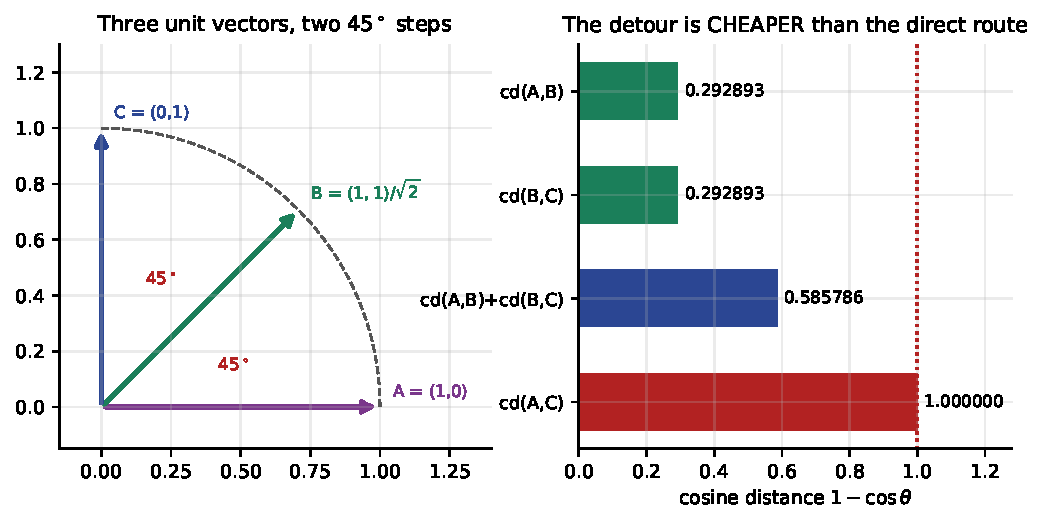
\includegraphics[width=0.95\textwidth]{triangle_violation.pdf}
      \end{center}
      \small Cosine distance fails too: two $45^\circ$ steps cost
      $0.292893$ each, the one $90^\circ$ step costs $1$. \textbf{The detour
      is cheaper than the direct route.} The repair is the \emph{angular}
      distance $\arccos(\cos\theta)/\pi$: $0.25+0.25 = 0.5$ exactly.
    \end{column}
  \end{columns}
\end{frame}

\begin{frame}[fragile,shrink=4]{And one that is not even symmetric}
\begin{lstlisting}
kl = lambda u, v: np.sum(u * np.log2(u / v))
p, q = np.array([0.5, 0.3, 0.2]), np.array([0.2, 0.4, 0.4])
\end{lstlisting}
\begin{outblk}
KL(p||q) = 0.336453   KL(q||p) = 0.301629   difference 0.034823
\end{outblk}
  \vspace{0.2em}
\begin{outblk}
measure                  d>=0  d(i,i)=0  symmetry  triangle
Euclidean                 yes       yes       yes       yes
Manhattan                 yes       yes       yes       yes
Minkowski p>=1            yes       yes       yes       yes
Chebyshev                 yes       yes       yes       yes
squared Euclidean         yes       yes       yes        NO
cosine distance           yes       no*       yes        NO
Jaccard distance          yes       yes       yes       yes
simple matching dist      yes       yes       yes       yes
KL divergence             yes       yes        NO        NO
\end{outblk}
  \begin{center}
    \small $*$ cosine distance is $0$ for any two \emph{parallel} vectors,
    not only equal ones: $\mathrm{cd}((1,2),(2,4)) = 0.000000$.
  \end{center}
\end{frame}

% =====================================================================
\section[Minkowski]{Numeric attributes: the Minkowski family}
\label{sec:mink}

\begin{frame}{One formula, one dial}
  \begin{exampleblock}{}
    \centering\large
    $\displaystyle d_p(x,y) = \Big( \sum_{f=1}^{m} |x_f - y_f|^p
    \Big)^{1/p}, \qquad p \ge 1$
  \end{exampleblock}
  \vspace{0.3em}
  \begin{columns}[T]
    \begin{column}{0.32\textwidth}
      \begin{block}{$p = 1$}
        \textbf{Manhattan}, city-block, $L_1$. Add the gaps up.
      \end{block}
    \end{column}
    \begin{column}{0.32\textwidth}
      \begin{block}{$p = 2$}
        \textbf{Euclidean}, $L_2$. The straight line. The default
        everywhere.
      \end{block}
    \end{column}
    \begin{column}{0.32\textwidth}
      \begin{block}{$p \to \infty$}
        \textbf{Chebyshev}, supremum, $L_\infty$. Only the single largest
        gap survives.
      \end{block}
    \end{column}
  \end{columns}
  \vspace{0.4em}
  \begin{center}
    \small $p$ controls \emph{how much a single bad attribute is punished}.
    Large $p$: one large disagreement dominates. $p=1$: it does not.
  \end{center}
\end{frame}

\begin{frame}[shrink=5]{By hand: one pair, four distances}
  \begin{exampleblock}{$x = (1,2)$, \quad $y = (4,6)$, \quad componentwise
    gaps $3$ and $4$}
    \begin{align*}
      d_1 &= |3| + |4| = \mathbf{7} \\[0.15em]
      d_2 &= \sqrt{3^2 + 4^2} = \sqrt{9+16} = \sqrt{25} = \mathbf{5}
        \quad \text{(the 3--4--5 triangle)} \\[0.15em]
      d_3 &= (3^3 + 4^3)^{1/3} = (27 + 64)^{1/3} = 91^{1/3}
        = \mathbf{4.497941} \\[0.15em]
      d_\infty &= \max(3, 4) = \mathbf{4}
    \end{align*}
  \end{exampleblock}
  \begin{center}
    \small Notice the order: $7 > 5 > 4.498 > 4$. That is general ---
    $d_1 \ge d_2 \ge d_3 \ge \cdots \ge d_\infty$ for every pair of points,
    always. Verified on $400$ random pairs in $\mathbb{R}^5$: all three
    inequalities hold in $400/400$ cases.
  \end{center}
\end{frame}

\begin{frame}[fragile,shrink=3]{The same thing in code}
\begin{lstlisting}
from scipy.spatial.distance import cityblock, euclidean, minkowski, chebyshev
x, y = np.array([1., 2.]), np.array([4., 6.])
for p in [1, 1.5, 2, 3, 4, 6, 8, 12, 20, 50, 100]:
    print(p, minkowski(x, y, p=p))
\end{lstlisting}
\begin{outblk}
     p      d_p(x,y)
     1      7.000000        6      4.110704
   1.5      5.584250        8      4.047992
     2      5.000000       12      4.010409
     3      4.497941       20      4.000633
     4      4.284572       50      4.000000
                          inf      4.000000
\end{outblk}
  \begin{center}
    \small The limit is $\max_f |x_f - y_f| = 4$, reached to six decimal
    places by $p = 50$. Chebyshev is not a separate idea; it is the end of
    the dial.
  \end{center}
\end{frame}

\begin{frame}[shrink=14]{Drawn: what the dial actually does}
  \begin{columns}[T]
    \begin{column}{0.5\textwidth}
      \begin{center}
        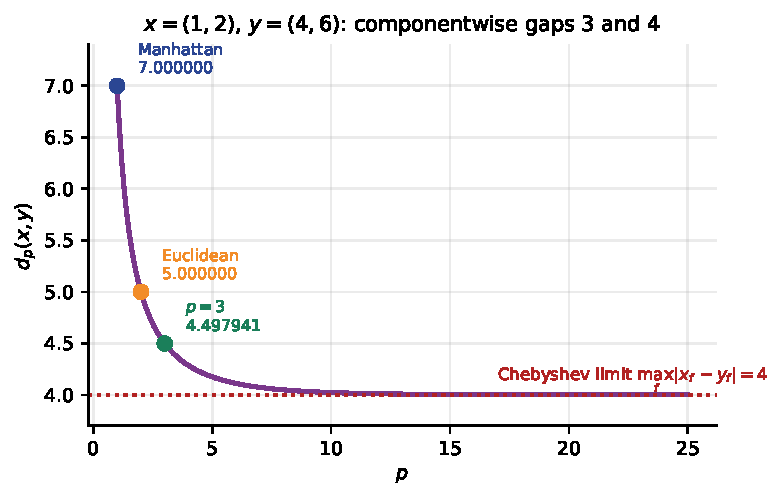
\includegraphics[width=0.94\textwidth]{minkowski_p.pdf}
      \end{center}
      \small Strictly decreasing in $p$, flattening onto the Chebyshev
      limit. Nothing is special about $p=2$ except habit.
    \end{column}
    \begin{column}{0.46\textwidth}
      \begin{center}
        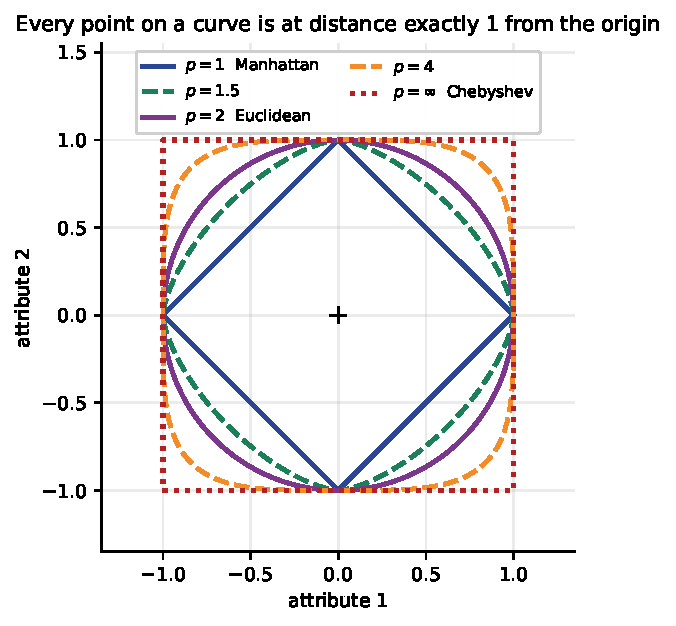
\includegraphics[width=0.62\textwidth]{unit_balls.pdf}
      \end{center}
      \small Every point on a curve is at distance \textbf{exactly 1} from
      the centre. Along the diagonal the two attributes disagree equally:
      $p=1$ pulls that direction in tightest, $p=\infty$ pushes it furthest
      out.
    \end{column}
  \end{columns}
  \begin{center}
    \small \textbf{Large $p$ forgives spreading a disagreement across
    attributes; $p=1$ does not care how it is spread.}
  \end{center}
\end{frame}

\begin{frame}[fragile,shrink=14]{Predict first \#1 --- which point is nearer?}
  \begin{exampleblock}{}
    \centering
    Query $q = (0,0)$. Candidate $u = (3,3)$ --- disagrees a little on both
    attributes. Candidate $v = (4.5, 0)$ --- disagrees a lot on one.\\[0.3em]
    \textbf{Which is $q$'s nearest neighbour? Commit before you look.}
  \end{exampleblock}
\onslide<2->
\begin{outblk}
metric           d(q,u)     d(q,v)   nearest
Manhattan      6.000000   4.500000   v
Euclidean      4.242641   4.500000   u
Minkowski3     3.779763   4.500000   u
Chebyshev      3.000000   4.500000   u
\end{outblk}
  \onslide<3->{%
  \begin{alertblock}{The answer is: it depends, and that is the point}
    Same data, same query, \textbf{different neighbour}. $p$ is not a
    tuning detail --- it encodes what you mean by ``alike''. If a customer
    who is a bit unusual on every attribute should count as more normal than
    one who is wildly unusual on a single attribute, you want large $p$.
  \end{alertblock}}
\end{frame}

% =====================================================================
\section[Cosine]{Cosine similarity against Euclidean distance}
\label{sec:cos}

\begin{frame}[shrink=10]{By hand: the pair that breaks the tie}
  \begin{exampleblock}{}
    \centering
    $\displaystyle \cos(x,y) = \frac{x \cdot y}{\|x\| \, \|y\|}$
    \quad --- the cosine of the angle. Range $[0,1]$ for count data.
    $\cos(x, kx) = 1$ for every $k > 0$: \textbf{length is discarded}.
  \end{exampleblock}
  \begin{exampleblock}{$A = (1,2)$, \quad $B = (10,20) = 10A$, \quad
    $C = (2,1)$}
    \[
      d(A,B) = \sqrt{9^2 + 18^2} = \sqrt{405} = 20.124612
      \qquad
      d(A,C) = \sqrt{1^2 + 1^2} = \sqrt{2} = 1.414214
    \]
    \[
      \cos(A,B) = \frac{10 + 40}{\sqrt5 \cdot \sqrt{500}}
      = \frac{50}{50} = 1.000000
      \qquad
      \cos(A,C) = \frac{2 + 2}{\sqrt5 \cdot \sqrt5} = \frac{4}{5} = 0.800000
    \]
  \end{exampleblock}
  \begin{center}
    \small \textbf{Euclidean} says $C$ is $A$'s nearest neighbour, by a
    factor of fourteen. \textbf{Cosine} says $B$ \emph{is} $A$, and $C$ is
    $36.87^\circ$ away. Neither is wrong; they answer different questions.
  \end{center}
\end{frame}

\begin{frame}[shrink=14]{Drawn: the disagreement}
  \begin{center}
    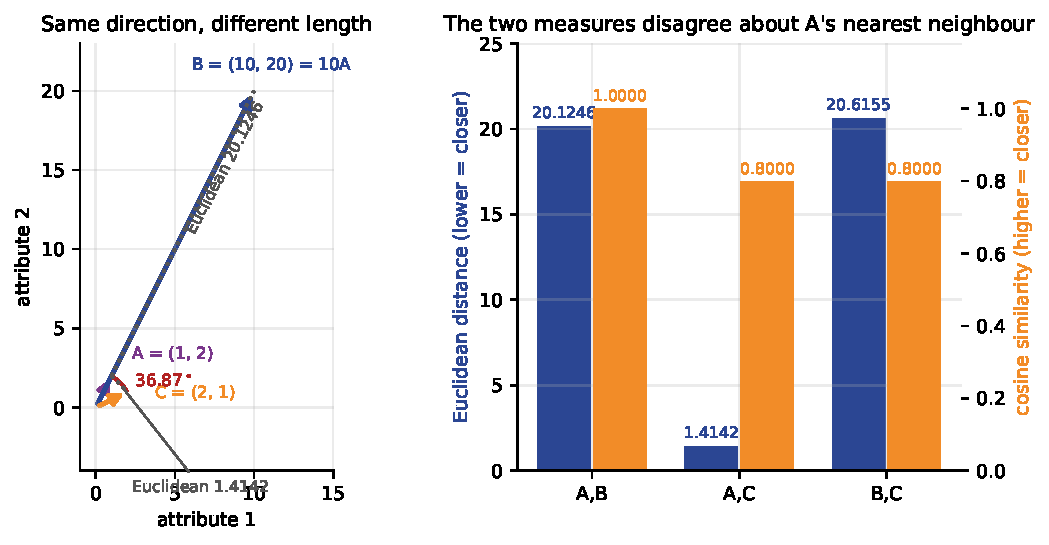
\includegraphics[width=0.76\textwidth]{cosine_vs_euclidean.pdf}
  \end{center}
  \vspace{-0.4em}
  \begin{center}
    \small The bars point in opposite directions: for Euclidean, lower is
    closer; for cosine, higher is closer. $A,B$ is the best possible cosine
    score and the second-worst Euclidean score in the same picture.\\
    \small \textbf{If magnitude carries information you have just discarded
    it; if magnitude is a nuisance, you have just removed it on purpose.}
  \end{center}
\end{frame}

\begin{frame}[fragile,shrink=14]{Predict first \#2 --- three documents}
  \begin{exampleblock}{}
    \centering
    \texttt{d1} $= [1,2,1,0,4]$ \quad
    \texttt{d2} $= [10,20,10,0,40]$ \quad
    \texttt{d3} $= [0,1,0,3,4]$\\[0.25em]
    \small \texttt{d2} is \texttt{d1} with every count multiplied by ten ---
    the same note, ten times as long. \texttt{d3} is a different note of the
    same length as \texttt{d1}.\\[0.3em]
    \textbf{Under Euclidean distance, which pair is closest?}
  \end{exampleblock}
\onslide<2->
\begin{outblk}
doc            doc                euclid     cosine
d1 short note  d2 long paper     42.2137     1.0000
d1 short note  d3 short note      3.4641     0.7526
d2 long paper  d3 short note     43.1972     0.7526
\end{outblk}
  \onslide<3->{%
  \begin{alertblock}{Euclidean pairs the two short documents}
    \texttt{d1} and \texttt{d3} are $3.46$ apart because they are both
    \emph{short}, not because they are about the same thing. \texttt{d1} and
    \texttt{d2} --- literally the same document --- are $42.21$ apart. On
    text, Euclidean distance clusters by length. \textbf{This is why text is
    the canonical cosine application.}
  \end{alertblock}}
\end{frame}

\begin{frame}[fragile]{The bridge: normalise the rows and they are the same}
  \begin{exampleblock}{}
    \centering\large
    $\displaystyle \Big\| \tfrac{a}{\|a\|} - \tfrac{b}{\|b\|} \Big\|^2
     = 2\big(1 - \cos(a,b)\big)$
  \end{exampleblock}
\begin{lstlisting}
uh, vh = u / np.linalg.norm(u), v / np.linalg.norm(v)
print(np.sum((uh - vh)**2), 2 * (1 - cosine_similarity([u], [v])[0, 0]))
\end{lstlisting}
\begin{outblk}
A,B    ||ahat-bhat||^2 = 0.0000000000   2(1-cos) = 0.0000000000   diff 2.22e-16
A,C    ||ahat-bhat||^2 = 0.4000000000   2(1-cos) = 0.4000000000   diff 3.89e-16
B,C    ||ahat-bhat||^2 = 0.4000000000   2(1-cos) = 0.4000000000   diff 1.67e-16
\end{outblk}
  \begin{center}
    \small So ``use cosine'' and ``$L_2$-normalise every row, then use
    Euclidean'' are \textbf{the same procedure}. That is often the easier
    one to implement, because every library takes Euclidean.
  \end{center}
\end{frame}

% =====================================================================
\section[Binary]{Binary attributes}
\label{sec:bin}

\begin{frame}{The $2 \times 2$ contingency table}
  \begin{columns}[T]
    \begin{column}{0.46\textwidth}
      \begin{center}
        \begin{tabular}{cc|cc|c}
          & & \multicolumn{2}{c|}{object $j$} & \\
          & & $1$ & $0$ & sum \\ \hline
          object & $1$ & $q$ & $r$ & $q+r$ \\
          $i$    & $0$ & $s$ & $t$ & $s+t$ \\ \hline
                 & sum & $q+s$ & $r+t$ & $p$
        \end{tabular}
      \end{center}
      \vspace{0.3em}
      \small $p = q+r+s+t$ is the number of attributes.
    \end{column}
    \begin{column}{0.5\textwidth}
      \begin{block}{The four counts}
        $q$ --- both $1$ (a shared \emph{presence})\\
        $r$ --- $i$ has it, $j$ does not\\
        $s$ --- $j$ has it, $i$ does not\\
        $t$ --- both $0$ (a shared \emph{absence})
      \end{block}
      \begin{alertblock}{One question decides everything}
        \textbf{Is $t$ evidence of similarity?}\\
        Two patients who both tested negative for forty rare diseases ---
        are they alike?
      \end{alertblock}
    \end{column}
  \end{columns}
\end{frame}

\begin{frame}[shrink=11]{Two answers, two coefficients}
  \begin{columns}[T]
    \begin{column}{0.48\textwidth}
      \begin{exampleblock}{Symmetric attributes}
        Both outcomes equally informative --- \texttt{gender}, coin flips,
        \texttt{is\_urban}.
        \[ \mathrm{SMC}(i,j) = \frac{q+t}{q+r+s+t} \]
        \[ d(i,j) = \frac{r+s}{q+r+s+t} \]
        \small The \textbf{simple matching coefficient}. Counts $t$.
      \end{exampleblock}
    \end{column}
    \begin{column}{0.48\textwidth}
      \begin{exampleblock}{Asymmetric attributes}
        One outcome rare and informative --- a positive test, a purchase, a
        word occurring.
        \[ J(i,j) = \frac{q}{q+r+s} \]
        \[ d(i,j) = \frac{r+s}{q+r+s} \]
        \small The \textbf{Jaccard coefficient}. Ignores $t$ entirely.
      \end{exampleblock}
    \end{column}
  \end{columns}
  \begin{center}
    \small The only difference is whether $t$ appears in the denominator.
    That one term is the whole examinable distinction.
  \end{center}
\end{frame}

\begin{frame}{By hand: three patients, six binary tests}
  \begin{center}
    \small
    \begin{tabular}{lcccccc}
      \toprule
      & fever & cough & test1 & test2 & test3 & test4 \\
      \midrule
      Jack & 1 & 0 & 1 & 0 & 0 & 0 \\
      Jim  & 1 & 1 & 0 & 0 & 0 & 0 \\
      Mary & 1 & 0 & 1 & 0 & 1 & 0 \\
      \bottomrule
    \end{tabular}
  \end{center}
  \vspace{0.3em}
  \begin{exampleblock}{Jack against Mary --- count, then divide}
    Both $1$: \texttt{fever}, \texttt{test1} $\Rightarrow q = 2$. \quad
    Jack $1$, Mary $0$: none $\Rightarrow r = 0$. \quad
    Mary $1$, Jack $0$: \texttt{test3} $\Rightarrow s = 1$. \quad
    Both $0$: \texttt{cough}, \texttt{test2}, \texttt{test4}
    $\Rightarrow t = 3$.
    \[
      \mathrm{SMC} = \frac{2+3}{6} = 0.8333
      \qquad
      J = \frac{2}{2+0+1} = \frac{2}{3} = 0.6667
    \]
  \end{exampleblock}
\end{frame}

\begin{frame}[fragile]{All three pairs, machine-checked}
\begin{lstlisting}
q = np.sum((u == 1) & (v == 1));  r = np.sum((u == 1) & (v == 0))
s = np.sum((u == 0) & (v == 1));  t = np.sum((u == 0) & (v == 0))
smc = (q + t) / (q + r + s + t);  jac = q / (q + r + s)
\end{lstlisting}
\begin{outblk}
pair           q   r   s   t |   SMC sim   SMC dis |   Jac sim   Jac dis
Jack,Jim       1   1   1   3 |    0.6667    0.3333 |    0.3333    0.6667
Jack,Mary      2   0   1   3 |    0.8333    0.1667 |    0.6667    0.3333
Jim,Mary       1   1   2   2 |    0.5000    0.5000 |    0.2500    0.7500
\end{outblk}
\begin{outblk}
Jack,Jim     scipy hamming 0.333333   scipy jaccard 0.666667
Jack,Mary    scipy hamming 0.166667   scipy jaccard 0.333333
Jim,Mary     scipy hamming 0.500000   scipy jaccard 0.750000
\end{outblk}
  \begin{center}
    \small For $0/1$ vectors \texttt{scipy}'s \texttt{hamming} --- the
    proportion of positions that disagree --- \textbf{is} the
    simple-matching dissimilarity $(r+s)/p$.
  \end{center}
\end{frame}

\begin{frame}[fragile,shrink=14]{Why the choice matters: pad with shared zeros}
  \begin{columns}[T]
    \begin{column}{0.42\textwidth}
\begin{outblk}
u = 1010, v = 1100, then
append k attributes that
are 0 for BOTH objects:
      k    SMC  Jaccard
      0  0.5000   0.3333
      4  0.7500   0.3333
     16  0.9000   0.3333
     96  0.9800   0.3333
    996  0.9980   0.3333
\end{outblk}
    \end{column}
    \begin{column}{0.56\textwidth}
      \begin{center}
        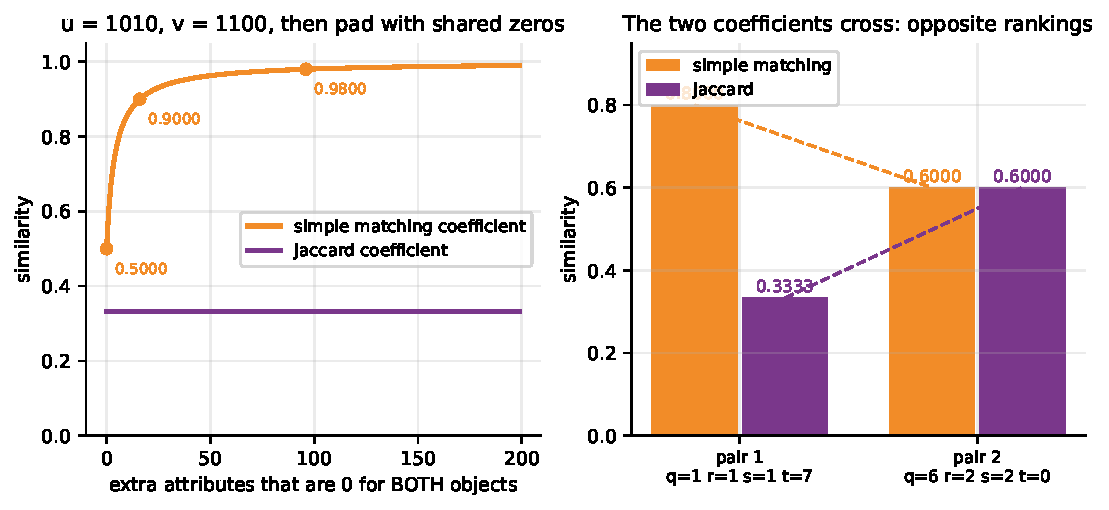
\includegraphics[width=0.97\textwidth]{binary_smc_jaccard.pdf}
      \end{center}
    \end{column}
  \end{columns}
  \begin{alertblock}{The market-basket argument}
    Add a thousand products \textbf{nobody bought} to the catalogue. Two
    shoppers who bought different things are now $99.8\%$ similar under
    simple matching, and unchanged under Jaccard. Adding items nobody bought
    cannot make two shoppers more alike.
  \end{alertblock}
\end{frame}

\begin{frame}[fragile,shrink=10]{Predict first \#3 --- the two coefficients cross}
  \begin{exampleblock}{}
    \centering\small
    \begin{tabular}{lll}
      \textbf{pair 1} & $u = 1100000000$ & $q=1, r=1, s=1, t=7$ \\
                      & $v = 1010000000$ & \\[0.3em]
      \textbf{pair 2} & $u = 1111111100$ & $q=6, r=2, s=2, t=0$ \\
                      & $v = 1111110011$ & \\
    \end{tabular}\\[0.4em]
    \textbf{Simple matching makes pair 1 the more similar
    ($0.8000$ vs $0.6000$). What does Jaccard say?}
  \end{exampleblock}
\onslide<2->
\begin{outblk}
simple matching: pair 1 (0.8000) is more similar than pair 2 (0.6000)
Jaccard:         pair 2 (0.6000) is more similar than pair 1 (0.3333)
\end{outblk}
  \onslide<3->{%
  \begin{alertblock}{Opposite rankings on the same data}
    Not a rounding difference --- a \textbf{reversal}. Any clustering built
    on these two coefficients will put different patients together. The
    decision ``is a shared absence evidence?'' is made once, before any
    algorithm runs, and it decides the answer.
  \end{alertblock}}
\end{frame}

\begin{frame}[fragile]{The $0/1$ coding is not a free choice}
\begin{outblk}
u = [1 1 1 0 0]   v = [1 0 0 0 0]
   q=1 r=2 s=0 t=2 ->  Jaccard sim 0.3333    SMC sim 0.6000
now swap the meaning of 0 and 1 on every attribute:
u = [0 0 0 1 1]   v = [0 1 1 1 1]
   q=2 r=0 s=2 t=1 ->  Jaccard sim 0.5000    SMC sim 0.6000
\end{outblk}
  \begin{columns}[T]
    \begin{column}{0.48\textwidth}
      \begin{block}{Simple matching: unchanged}
        $0.6000$ either way. It is symmetric in the two codes --- which is
        exactly what ``symmetric attribute'' means.
      \end{block}
    \end{column}
    \begin{column}{0.48\textwidth}
      \begin{alertblock}{Jaccard: $0.3333 \to 0.5000$}
        It counts only whichever value you coded as $1$. \textbf{Decide
        which outcome is the rare, informative one before you compute
        anything.}
      \end{alertblock}
    \end{column}
  \end{columns}
\end{frame}

% =====================================================================
\section[Nominal, ordinal]{Nominal and ordinal attributes}
\label{sec:nomord}

\begin{frame}{Nominal: categories with no order}
  \begin{exampleblock}{}
    \centering\large
    $\displaystyle d(i,j) = \frac{p - m}{p}$
  \end{exampleblock}
  \begin{center}
    \small $p$ = number of nominal attributes, $m$ = number on which
    $i$ and $j$ take the \emph{same} value. The \textbf{mismatch ratio}.
  \end{center}
  \vspace{0.2em}
  \begin{exampleblock}{Three objects, three nominal attributes}
    \small
    \begin{tabular}{lccc}
      \toprule
      & colour & shape & material \\ \midrule
      A & red & round & wood \\
      B & red & square & wood \\
      C & blue & square & metal \\ \bottomrule
    \end{tabular}
    \qquad
    \begin{tabular}{lccc}
      \toprule
      pair & $p$ & $m$ & $(p-m)/p$ \\ \midrule
      A,B & 3 & 2 & $1/3 = 0.333333$ \\
      A,C & 3 & 0 & $3/3 = 1.000000$ \\
      B,C & 3 & 1 & $2/3 = 0.666667$ \\ \bottomrule
    \end{tabular}
  \end{exampleblock}
\end{frame}

\begin{frame}[fragile,shrink=14]{The one-hot alternative --- equivalent, or not?}
\begin{outblk}
columns: colour=blue, colour=red, shape=round, shape=square, material=metal, material=wood
  A        0  1  1  0  0  1
  B        0  1  0  1  0  1
  C        1  0  0  1  1  0

pair        (p-m)/p      L1/(2p)   L1 one-hot   L2 one-hot
A,B        0.333333     0.333333     2.000000     1.414214
A,C        1.000000     1.000000     6.000000     2.449490
B,C        0.666667     0.666667     4.000000     2.000000
\end{outblk}
  \begin{columns}[T]
    \begin{column}{0.48\textwidth}
      \begin{block}{$L_1$: exactly the same measure}
        Each mismatch flips two dummy columns, so
        $L_1 = 2(p-m)$ and $L_1/(2p) = (p-m)/p$ to the last digit.
      \end{block}
    \end{column}
    \begin{column}{0.48\textwidth}
      \begin{alertblock}{$L_2$: same ranking, different numbers}
        $L_2 = \sqrt{2(p-m)}$. The extreme ratio is $3.0000$ for the
        mismatch ratio but only $1.7321$ for $L_2$ --- \textbf{Euclidean on
        dummies compresses the gaps by a square root.}
      \end{alertblock}
    \end{column}
  \end{columns}
\end{frame}

\begin{frame}[fragile,shrink=3]{Where one-hot stops agreeing --- a real reversal}
\begin{outblk}
20 rows, three nominal attributes.  Level frequencies:
  f1: {'a': 10, 'b': 10}    f2: {'P': 10, 'Q': 10}    f3: {'u': 19, 'w': 1}
column standard deviations (sqrt(pi(1-pi)) for a dummy):
  0.5000  0.5000  0.5000  0.5000  0.2179  0.2179

obj  f1   f2   f3   | mismatches |      (p-m)/p |     z-dummy L2
x0   a    P    u    |          0 |     0.000000 |       0.000000
xA   a    P    w    |          1 |     0.333333 |       6.488857
xB   b    Q    u    |          2 |     0.666667 |       4.000000
\end{outblk}
  \begin{alertblock}{Ranking flip}
    The mismatch ratio says \texttt{xA} (one mismatch) is nearer to
    \texttt{x0}. Standardised dummies say \texttt{xB} (two mismatches) is
    nearer. Nothing in the data changed --- only the \emph{frequency} of the
    level \texttt{'w'}, which occurs once in twenty. \textbf{A rare category
    buys influence the mismatch ratio never granted it.}
  \end{alertblock}
\end{frame}

\begin{frame}[shrink=14]{Ordinal: categories with an order}
  \begin{exampleblock}{}
    \centering\large
    rank $r \in \{1,\dots,M\}$
    \quad$\longrightarrow$\quad
    $\displaystyle z = \frac{r-1}{M-1} \in [0,1]$
    \quad$\longrightarrow$\quad treat as numeric
  \end{exampleblock}
  \begin{columns}[T]
    \begin{column}{0.46\textwidth}
      \begin{exampleblock}{Two scales, and a pair}
        \small
        $M=5$: poor $0$, fair $0.25$, good $0.5$, very good $0.75$,
        excellent $1$. \quad $M=3$: junior $0$, mid $0.5$, senior
        $1$.\\[0.4em]
        $P$ = (excellent, senior) $\to (1.00, 1.00)$;\quad
        $Q$ = (good, junior) $\to (0.50, 0.00)$.\\[0.3em]
        $|1.00-0.50| = 0.50$, $|1.00-0.00| = 1.00$;
        Euclidean $\sqrt{1.25} = 1.118034$; mean absolute gap
        $0.750000$.
      \end{exampleblock}
    \end{column}
    \begin{column}{0.5\textwidth}
      \begin{block}{Why divide by $M-1$}
        So scales of different length are commensurable. A three-level and a
        seven-level attribute both span exactly $[0,1]$, and neither
        dominates the sum by accident.
      \end{block}
      \begin{center}
        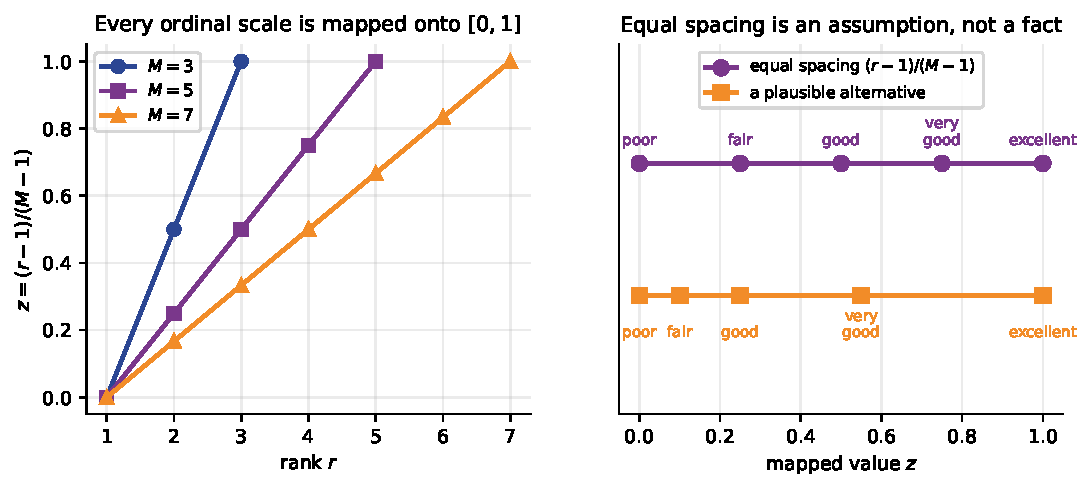
\includegraphics[width=0.92\textwidth]{ordinal_map.pdf}
      \end{center}
    \end{column}
  \end{columns}
  \begin{center}
    \small Equal spacing says poor-vs-fair and very-good-vs-excellent are
    the same distance apart. \textbf{That is an assumption you should be
    willing to defend.}
  \end{center}
\end{frame}

% =====================================================================
\section[Mixed]{Mixed attribute types}
\label{sec:mixed}

\begin{frame}[shrink=4]{Gower: one weighted average across the types}
  \begin{exampleblock}{}
    \centering\large
    $\displaystyle d(i,j) =
      \frac{\sum_{f=1}^{p} \delta_f^{(ij)} \, d_f^{(ij)}}
           {\sum_{f=1}^{p} \delta_f^{(ij)}}$
  \end{exampleblock}
  \begin{columns}[T]
    \begin{column}{0.5\textwidth}
      \begin{block}{$d_f^{(ij)}$ --- one number per attribute, in $[0,1]$}
        \small
        \textbf{numeric}: $|x_{if}-x_{jf}| / R_f$, $R_f$ the range\\
        \textbf{nominal / symmetric binary}: $0$ if equal, else $1$\\
        \textbf{asymmetric binary}: $0$ if equal, else $1$\\
        \textbf{ordinal}: map to $z$, then $|z_{if} - z_{jf}|$
      \end{block}
    \end{column}
    \begin{column}{0.46\textwidth}
      \begin{alertblock}{$\delta_f^{(ij)}$ --- the indicator, and it does work}
        $\delta_f = 0$ when the attribute is missing for either object,
        \textbf{or} when the attribute is asymmetric binary and both objects
        are $0$. Otherwise $\delta_f = 1$.\\[0.3em]
        A dropped attribute leaves \emph{both} the numerator and the
        denominator.
      \end{alertblock}
    \end{column}
  \end{columns}
\end{frame}

\begin{frame}[shrink=4]{By hand: four applicants, four attribute types}
  \begin{center}
    \small
    \begin{tabular}{lrrllccc}
      \toprule
      id & age & exp & degree & city & car & python & patent \\
      \midrule
      A & 24 & 2 & BTech & Dehradun & 1 & 1 & 0 \\
      B & 29 & 6 & MTech & Dehradun & 0 & 1 & 0 \\
      C & 41 & 18 & PhD & Mumbai & 1 & 0 & 1 \\
      D & 26 & 3 & BTech & Delhi & 0 & 1 & 0 \\
      \bottomrule
    \end{tabular}
  \end{center}
  \begin{exampleblock}{$d(A,B)$, attribute by attribute}
    \small
    Ranges: $R_{\text{age}} = 41-24 = 17$, $R_{\text{exp}} = 18-2 = 16$.
    Ordinal: BTech $0$, MTech $0.5$, PhD $1$.
    \[
      \underbrace{\tfrac{5}{17}}_{0.294118}
      + \underbrace{\tfrac{4}{16}}_{0.250000}
      + \underbrace{|0-0.5|}_{0.500000}
      + \underbrace{0}_{\text{same city}}
      + \underbrace{1}_{\text{car } 1\text{ vs }0}
      + \underbrace{0}_{\text{python }1,1}
      + \underbrace{\text{skipped}}_{\text{patent } 0,0}
      = 2.044118
    \]
    \[ d(A,B) = 2.044118 \,/\, 6 = \mathbf{0.340686} \]
  \end{exampleblock}
\end{frame}

\begin{frame}[fragile]{Where the asymmetric rule bites: $d(B,D)$}
\begin{outblk}
attribute f            delta_f        d_f      delta*d
age (numeric)                1   0.176471     0.176471
experience (numeric)         1   0.187500     0.187500
degree (ordinal)             1   0.500000     0.500000
city (nominal)               1   1.000000     1.000000
car (asym binary)            0   0.000000     0.000000
python (asym binary)         1   0.000000     0.000000
patent (asym binary)         0   0.000000     0.000000
SUM                          5                1.863971
d = 1.863971 / 5 = 0.372794
\end{outblk}
  \begin{center}
    \small \textbf{Two} attributes were dropped: neither B nor D owns a car,
    neither holds a patent. The denominator is $5$, not $7$. Divide by $7$
    and you get $0.266282$ --- a different answer and a wrong one.
  \end{center}
\end{frame}

\begin{frame}[shrink=10]{Drawn: the contributions and the matrix}
  \begin{center}
    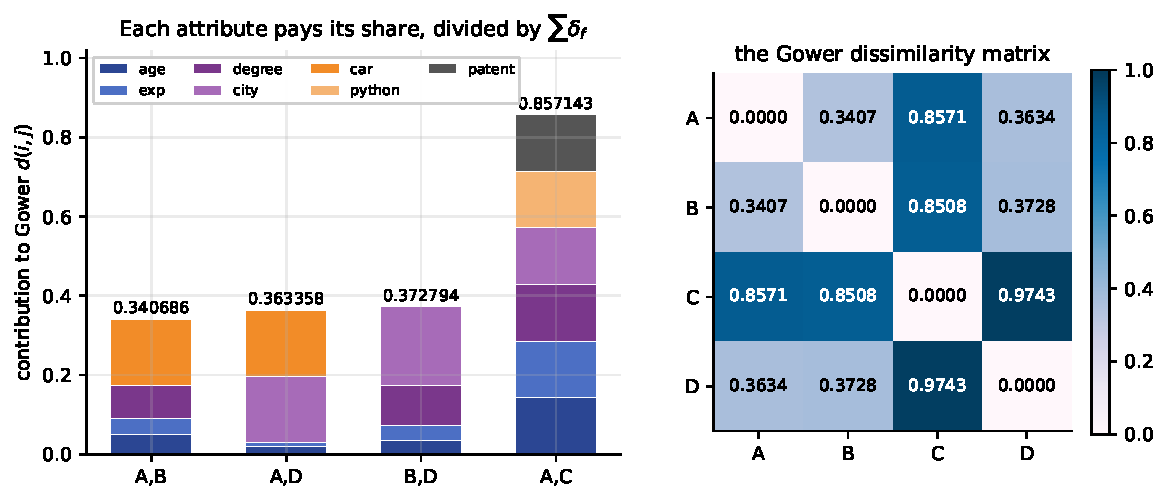
\includegraphics[width=0.86\textwidth]{mixed_gower.pdf}
  \end{center}
  \vspace{-0.4em}
  \begin{center}
    \small Nearest to A: \textbf{B $0.340686$} then \textbf{D $0.363358$}
    then C $0.857143$. B and D are separated by $0.022672$ --- one attribute
    either way would swap them, which is why the weighting is worth arguing
    about.
  \end{center}
\end{frame}

\begin{frame}[fragile,shrink=12]{Drop the type handling and the answer changes}
\begin{lstlisting}
E = [[age, exp, DEGREE.index(deg), cities.index(city), car, py, pat] ...]
Draw = squareform(pdist(E, "euclidean"))
\end{lstlisting}
\begin{outblk}
nearest to A, raw Euclidean : D
nearest to A, z-scored      : D
nearest to A, Gower         : B
\end{outblk}
  \begin{alertblock}{What label-encoding quietly asserted}
    That \texttt{city} is a number on which Delhi $(0) <$ Dehradun $(1) <$
    Mumbai $(2)$, so Delhi is ``closer to'' Dehradun than to Mumbai by
    exactly one unit. Nobody chose that ordering, the data does not support
    it, and it changed which applicant is A's nearest neighbour.
  \end{alertblock}
  \begin{center}
    \small \texttt{LabelEncoder} on a nominal column is the single commonest
    silent bug in student clustering code.
  \end{center}
\end{frame}

% =====================================================================
\section[Standardisation]{Standardisation changes the answer}
\label{sec:std}

\begin{frame}[fragile,shrink=3]{Predict first \#4 --- who is row 1's neighbour?}
  \begin{exampleblock}{}
    \centering\small
    Ten customers. Two attributes: annual fee (in rupees, around $50\,000$)
    and a usage ratio in $[0,1]$.
    Query is row 1: fee $50\,000$, usage $0.50$.\\[0.3em]
    Row 2 is (\,$50\,300$, $0.90$\,). Row 4 is (\,$49\,500$, $0.42$\,).\\[0.3em]
    \textbf{Which one is nearer? Now: does your answer survive
    standardising?}
  \end{exampleblock}
\onslide<2->
\begin{outblk}
 row          fee    usage |        d raw   d z-scored
   1        50000     0.50 |     0.000000     0.000000   <- query
   2        50300     0.90 |   300.000267     1.823190
   4        49500     0.42 |   500.000006     0.467002
nearest neighbour, raw      : row 2  (d = 300.000267)
nearest neighbour, z-scored : row 4  (d = 0.467002)
\end{outblk}
  \onslide<3->{%
  \begin{center}
    \small \textbf{Different row.} And the share of raw squared distance
    carried by the fee column, over all nine other rows: mean
    $\mathbf{1.000000}$ to six decimal places. The usage column was not
    consulted.
  \end{center}}
\end{frame}

\begin{frame}[fragile,shrink=12]{Drawn: the same ten points, twice --- and on real data}
  \begin{center}
    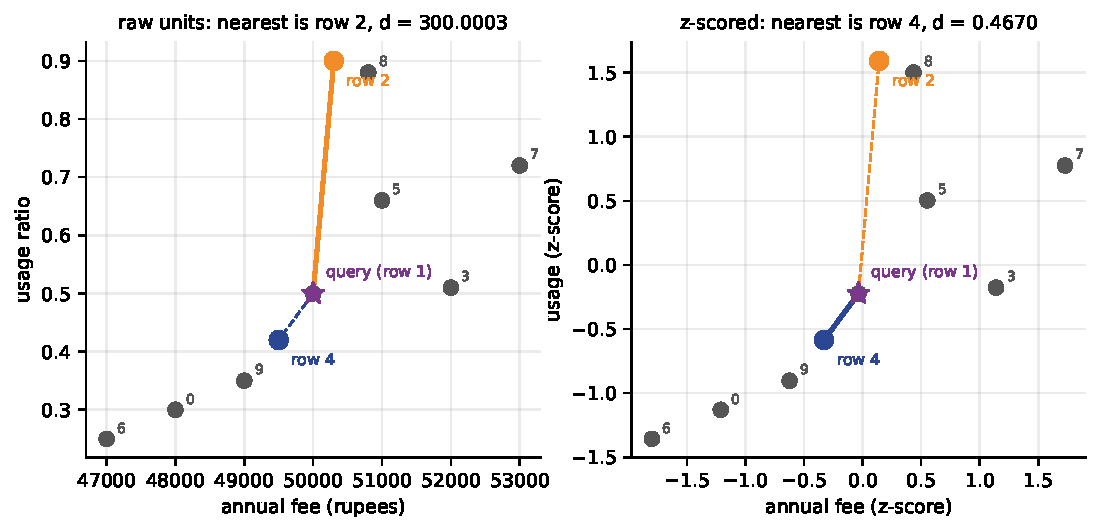
\includegraphics[width=0.70\textwidth]{standardisation_flip.pdf}
  \end{center}
  \vspace{-0.3em}
\begin{outblk}
wine: 178 rows, 13 features
rows whose nearest neighbour CHANGES IDENTITY under z-scoring: 168 / 178 (94.4%)
one column, proline (variance 98609.6), carries 0.997738 of the total
raw squared distance.
\end{outblk}
  \begin{center}
    \small An unscaled distance is a distance in whichever column has the
    biggest numbers.
  \end{center}
\end{frame}

\begin{frame}[fragile]{By hand: z-score against mean absolute deviation}
  \begin{exampleblock}{$x = 1, 2, 3, 4, 100$. Mean $= 22$.}
    \small
    $\sigma = \sqrt{\tfrac{21^2+20^2+19^2+18^2+78^2}{5}}
      = \sqrt{\tfrac{7610}{5}} = \sqrt{1522} = 39.012818$\\[0.3em]
    $s = \tfrac{21+20+19+18+78}{5} = \tfrac{156}{5} = 31.200000$
    \quad (the \textbf{mean absolute deviation})
  \end{exampleblock}
\begin{outblk}
gap between x=1 and x=2 after scaling:
  by sd  0.025633       by mad  0.032051       ratio 1.2504
the outlier's own score:  sd 1.9993   mad 2.5000
\end{outblk}
  \begin{center}
    \small $\sigma$ is inflated by the \emph{square} of the outlier's
    deviation; the mean absolute deviation only linearly. So $\sigma$
    crushes the four ordinary points together, and MAD scaling leaves them
    $\mathbf{25.0\%}$ further apart from each other.
  \end{center}
\end{frame}

\begin{frame}[fragile,shrink=14]{Drawn --- and reported honestly}
  \begin{center}
    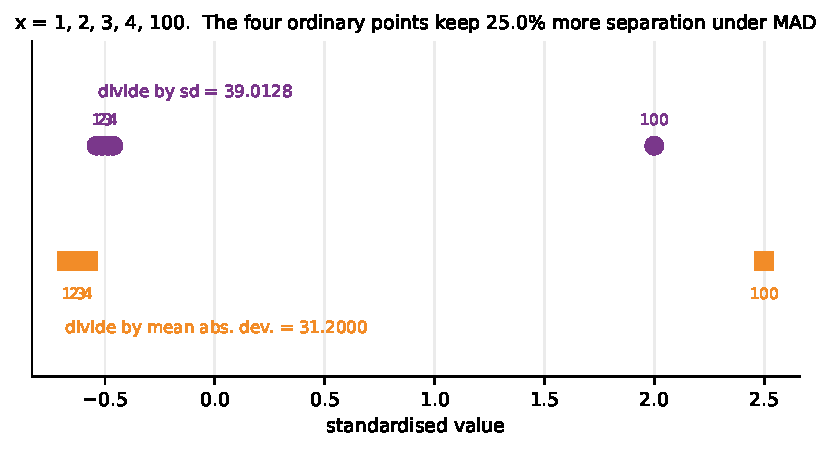
\includegraphics[width=0.54\textwidth]{zscore_vs_mad.pdf}
  \end{center}
  \vspace{-0.3em}
\begin{outblk}
dataset        column                             sd        mad   sd/mad
breast_cancer  area error                    45.4510    27.1965   1.6712
wine           od280/od315_of_diluted_wines     0.7080     0.6117   1.1573
iris           petal length (cm)              1.7594     1.5627   1.1258
\end{outblk}
  \begin{center}
    \small For a Gaussian column $\sigma/s \to \sqrt{\pi/2} = 1.2533$. Every
    \texttt{wine} and \texttt{iris} column sits near that, so there the two
    choices barely differ. \textbf{MAD scaling earns its keep when the tail
    is real} --- as on the \texttt{breast\_cancer} error columns.
  \end{center}
\end{frame}

% =====================================================================
\section[Centroids]{Cluster centroid, medoid and cluster distances}
\label{sec:cent}

\begin{frame}{Three ways to name ``the middle''}
  \begin{columns}[T]
    \begin{column}{0.32\textwidth}
      \begin{block}{Centroid}
        The componentwise mean $\bar{c} = \tfrac1n \sum_i x_i$.\\[0.3em]
        \small Minimises $\sum_i \|x_i - c\|^2$. Usually \textbf{not} a data
        point. Needs numeric attributes.
      \end{block}
    \end{column}
    \begin{column}{0.32\textwidth}
      \begin{block}{Medoid}
        The object with the smallest total distance to the rest.\\[0.3em]
        \small \textbf{Is} a data point. Works with any dissimilarity
        matrix, including Gower.
      \end{block}
    \end{column}
    \begin{column}{0.32\textwidth}
      \begin{block}{Mode}
        The most frequent value per attribute.\\[0.3em]
        \small For purely nominal data, where means are meaningless
        (``the average colour'').
      \end{block}
    \end{column}
  \end{columns}
  \vspace{0.4em}
  \begin{exampleblock}{}
    \centering
    This distinction is the whole difference between $k$-means and
    $k$-medoids, and it is why $k$-medoids can cluster mixed-type data and
    $k$-means cannot.
  \end{exampleblock}
\end{frame}

\begin{frame}{By hand: a three-point cluster}
  \begin{exampleblock}{$A = \{(1,1),\, (2,1),\, (1,2)\}$}
    \small
    \textbf{Centroid} $= \big(\tfrac{1+2+1}{3}, \tfrac{1+1+2}{3}\big)
      = (1.333333,\ 1.333333)$ --- not one of the three points.\\[0.4em]
    \textbf{Medoid} --- total distance to the others:
    \begin{center}
      \begin{tabular}{lccc}
        \toprule
        point & to the others & & total \\ \midrule
        $(1,1)$ & $1.000000$ & $1.000000$ & $\mathbf{2.000000}$ \\
        $(2,1)$ & $1.000000$ & $1.414214$ & $2.414214$ \\
        $(1,2)$ & $1.000000$ & $1.414214$ & $2.414214$ \\ \bottomrule
      \end{tabular}
    \end{center}
    \textbf{Medoid} $= (1,1)$ --- and it \emph{is} one of the three points.
  \end{exampleblock}
\end{frame}

\begin{frame}[fragile]{The identity that makes the mean the right centre}
  \begin{exampleblock}{}
    \centering\large
    $\displaystyle \sum_{i} \|x_i - \bar{c}\|^2
     = \frac{1}{2n}\sum_i \sum_j \|x_i - x_j\|^2$
  \end{exampleblock}
\begin{outblk}
SSE(A) = sum_i ||x_i - centroid||^2          = 1.333333
       = (1/2n) sum_i sum_j ||x_i - x_j||^2  = 1.333333
difference 0.00e+00
  best grid point (1.3330, 1.3330), SSE 1.333334
\end{outblk}
  \begin{center}
    \small The right-hand side does not mention $\bar{c}$ at all, so the
    within-cluster scatter is a property of the \emph{pairwise distances}.
    A brute-force search over a fine grid finds the minimum exactly where
    the mean is --- which is \textbf{why $k$-means uses means}.
  \end{center}
\end{frame}

\begin{frame}[fragile]{By hand: distance between two clusters}
  \begin{columns}[T]
    \begin{column}{0.34\textwidth}
      \small
      $A = \{(1,1),(2,1),(1,2)\}$\\
      $B = \{(5,5),(6,5),(5,6)\}$\\[0.4em]
      Nine cross distances, all computed with Pythagoras.
    \end{column}
    \begin{column}{0.63\textwidth}
\begin{outblk}
             b1=(5,5)    b2=(6,5)    b3=(5,6)
a1=(1,1)     5.656854    6.403124    6.403124
a2=(2,1)     5.000000    5.656854    5.830952
a3=(1,2)     5.000000    5.830952    5.656854
\end{outblk}
    \end{column}
  \end{columns}
  \vspace{0.3em}
  \begin{exampleblock}{The four classical linkages}
    \small
    \textbf{single} (min) $= 5.000000$ \quad
    \textbf{complete} (max) $= 6.403124$ \quad
    \textbf{average} (mean of all nine) $= 5.715413$ \quad
    \textbf{centroid} $= \|(1.3333,1.3333) - (5.3333,5.3333)\|
      = 4\sqrt2 = 5.656854$
  \end{exampleblock}
\end{frame}

\begin{frame}[shrink=14]{Drawn: four ways to measure one gap}
  \begin{center}
    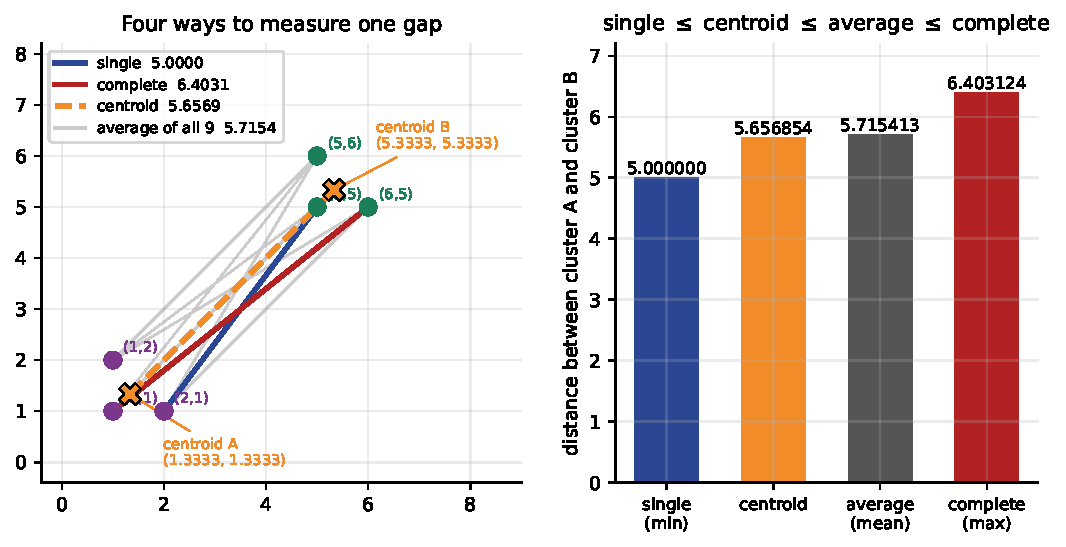
\includegraphics[width=0.76\textwidth]{linkage_distances.pdf}
  \end{center}
  \vspace{-0.4em}
  \begin{center}
    \small Ordering: single $5.0000 \le$ centroid $5.6569 \le$ average
    $5.7154 \le$ complete $6.4031$. Centroid $\le$ average always: the
    distance between the means is at most the mean of the distances
    (Jensen). Gap here $0.058559$.
  \end{center}
\end{frame}

\begin{frame}[fragile]{Ward: the fifth one, and it is not a distance}
\begin{outblk}
SSE(A) 1.333333 + SSE(B) 1.333333 = 2.666667
SSE(A union B)                = 50.666667
increase on merging           = 48.000000
closed form (nA nB/(nA+nB)) ||cA-cB||^2 = 48.000000   diff 1.42e-14
\end{outblk}
  \begin{columns}[T]
    \begin{column}{0.48\textwidth}
      \begin{block}{What Ward measures}
        Not how far apart the clusters are, but \textbf{how much
        within-cluster scatter merging them would create}. Here $48.000000$.
      \end{block}
    \end{column}
    \begin{column}{0.48\textwidth}
      \begin{alertblock}{Which is why}
        \texttt{scipy}'s \texttt{ward} reports $9.797959$ where the other
        four report numbers near $5.7$. Do \textbf{not} compare a Ward
        height with a single-linkage height. Different units.
      \end{alertblock}
    \end{column}
  \end{columns}
  \begin{center}
    \small \texttt{scipy.cluster.hierarchy.linkage} reproduces all four hand
    numbers exactly: $5.000000$, $6.403124$, $5.715413$, $5.656854$.
  \end{center}
\end{frame}

% =====================================================================
\section[Summary]{Does any of this actually change a clustering?}
\label{sec:summary}

\begin{frame}[fragile]{Predict first \#5 --- one algorithm, eight distances}
  \begin{exampleblock}{}
    \centering\small
    \texttt{AgglomerativeClustering(n\_clusters=3, linkage='average')} on
    \texttt{load\_wine}, scored against the true cultivar with the adjusted
    Rand index.\\[0.3em]
    \textbf{Rank these: Euclidean, Manhattan, Chebyshev, cosine --- raw and
    z-scored. Which combination wins?}
  \end{exampleblock}
\onslide<2->
\begin{outblk}
metric              ARI raw ARI z-scored
euclidean            0.2926      -0.0054
manhattan            0.3186       0.4730
chebyshev            0.2926      -0.0068
cosine               0.0535       0.7847
kmeans (L2sq)        0.3711       0.8975
\end{outblk}
  \onslide<3->{%
  \begin{center}
    \small From $\mathbf{0.0535}$ to $\mathbf{0.8975}$ --- and the algorithm
    never changed. Only the distance did.
  \end{center}}
\end{frame}

\begin{frame}[fragile,shrink=3]{Two honest footnotes on that table}
  \begin{columns}[T]
    \begin{column}{0.49\textwidth}
      \begin{alertblock}{Standardising made one row \emph{worse}}
        Average-linkage Euclidean fell from $0.2926$ to $-0.0054$.
\begin{outblk}
  raw       sizes [130, 42, 6]
  z-scored  sizes [174, 1, 3]
\end{outblk}
        Not a distance failure: average linkage peeled off outliers once
        standardising let the small-scale columns speak. \textbf{Choose the
        distance and the linkage together.}
      \end{alertblock}
    \end{column}
    \begin{column}{0.49\textwidth}
      \begin{block}{Cosine on raw wine did badly --- correctly}
        Raw wine's vector length \emph{is} proline, and proline separates
        the cultivars. Throwing the length away throws the signal away
        ($0.0535$). On text, where length is document length, throwing it
        away is exactly right.\\[0.3em]
        \small And Euclidean on $L_2$-normalised rows gives the identical
        partition: ARI $0.0535$ both ways.
      \end{block}
    \end{column}
  \end{columns}
\end{frame}

\begin{frame}[shrink=3]{Drawn: the whole argument in one chart}
  \begin{center}
    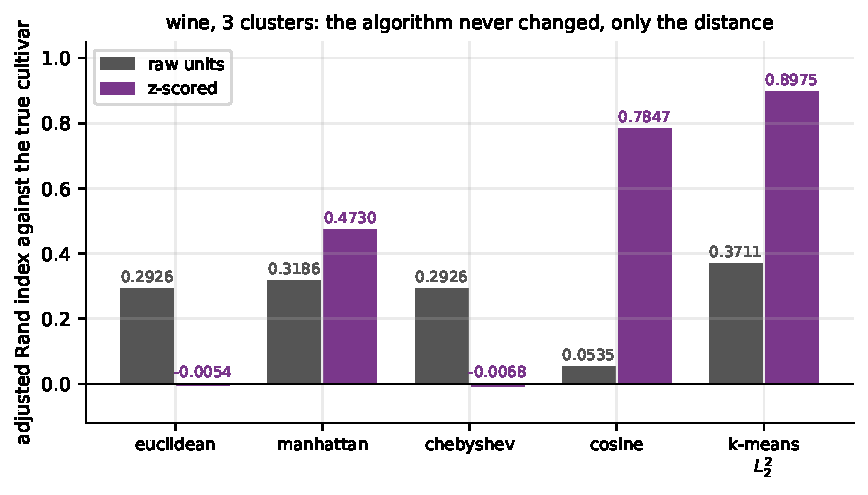
\includegraphics[width=0.62\textwidth]{wine_distance_choice.pdf}
  \end{center}
  \vspace{-0.3em}
  \begin{center}
    \small Ten bars. One algorithm. The spread from $-0.0068$ to $0.8975$ is
    entirely the distance and the scaling. \textbf{Nothing you do to the
    algorithm will recover a badly chosen distance.}
  \end{center}
\end{frame}

\begin{frame}{Summary --- twelve lines (1 of 2)}
  \begin{enumerate}
    \item A dissimilarity is a \textbf{metric} if it satisfies
      non-negativity, identity, symmetry and the triangle inequality.
      \textbf{Squared Euclidean} and \textbf{cosine distance} fail the
      triangle inequality; \textbf{KL divergence} fails symmetry.
    \item $d_p = (\sum_f |x_f-y_f|^p)^{1/p}$: $p{=}1$ Manhattan, $p{=}2$
      Euclidean, $p{\to}\infty$ Chebyshev. For $(1,2)$ and $(4,6)$:
      $\mathbf{7}$, $\mathbf{5}$, $4.497941$, $\mathbf{4}$.
    \item $d_1 \ge d_2 \ge \cdots \ge d_\infty$ always. Large $p$ punishes a
      single bad attribute; $p{=}1$ does not. On $q{=}(0,0)$,
      $u{=}(3,3)$, $v{=}(4.5,0)$ they pick different neighbours.
    \item Cosine measures direction and discards length.
      $A{=}(1,2)$, $B{=}10A$, $C{=}(2,1)$: Euclidean says $C$
      ($1.4142$ vs $20.1246$), cosine says $B$ ($1.0000$ vs $0.8000$).
    \item $\|\hat a - \hat b\|^2 = 2(1-\cos)$, so cosine \emph{is}
      Euclidean on $L_2$-normalised rows.
  \end{enumerate}
\end{frame}

\begin{frame}[shrink=14]{Summary --- twelve lines (2 of 2)}
  \begin{enumerate}
    \setcounter{enumi}{5}
    \item Binary: build $q, r, s, t$. \textbf{Simple matching}
      $(q{+}t)/p$ for symmetric attributes; \textbf{Jaccard} $q/(q{+}r{+}s)$
      for asymmetric. The question is whether a shared \emph{absence} is
      evidence.
    \item They can rank two pairs in \textbf{opposite orders}: $0.8000$ vs
      $0.6000$ against $0.3333$ vs $0.6000$. Padding with shared zeros
      drives simple matching to $0.9980$ and leaves Jaccard at $0.3333$.
    \item Nominal: $(p-m)/p$. One-hot with $L_1$ is \emph{exactly} the same
      measure; with $L_2$ the ranking survives but the gaps compress by a
      square root; with \emph{standardised} dummies the ranking can flip.
    \item Ordinal: $z = (r-1)/(M-1)$, then treat as numeric. Equal spacing
      is an assumption.
    \item Mixed: Gower, $\sum \delta_f d_f / \sum \delta_f$. A $0$--$0$ pair
      on an asymmetric binary attribute sets $\delta_f = 0$ and leaves both
      sums. $d(A,B) = \mathbf{0.340686}$, $d(B,D) = \mathbf{0.372794}$.
    \item Standardisation changes which object is nearest ---
      $\mathbf{94.4\%}$ of \texttt{wine} rows. MAD scaling is the robust
      alternative; $\sigma/s \to \sqrt{\pi/2} = 1.2533$ for a Gaussian
      column.
    \item Centroid $\ne$ medoid. Cluster distances: single $5.0000$,
      centroid $5.6569$, average $5.7154$, complete $6.4031$ --- in that
      order, always.
  \end{enumerate}
\end{frame}

\begin{frame}[fragile,shrink=14]{Before the next lecture}
  \begin{columns}[T]
    \begin{column}{0.48\textwidth}
      \begin{block}{Read and do}
        \texttt{notes.pdf} --- \textbf{ten practice questions with full
        worked solutions}, four of them pure hand computation. Rebuild the
        three-patient table with a pen, then $d(A,C)$ and $d(C,D)$ for the
        applicant table showing every $\delta_f$.
      \end{block}
      \begin{exampleblock}{The habit to take away}
        Before you cluster anything, write down for each column: its
        \textbf{type}, whether it is \textbf{symmetric}, and its
        \textbf{units}.
      \end{exampleblock}
    \end{column}
    \begin{column}{0.48\textwidth}
      \begin{alertblock}{What the matrix costs}
\begin{outblk}
         n              pairs   MB at 8 bytes
       150              11175             0.1
      1000             499500             4.0
     10000           49995000           400.0
    100000         4999950000         39999.6
\end{outblk}
        At a hundred thousand objects the dissimilarity matrix alone is
        \textbf{40 GB}. This is why the hierarchical methods of the next
        lecture are quadratic in memory, and why $k$-means --- which never
        forms the matrix --- scales further.
      \end{alertblock}
    \end{column}
  \end{columns}
  \begin{center}
    \small Materials: \texttt{\AMLRepoURL}
  \end{center}
  \slidesources{\AMLUnitVIISources}
\end{frame}

\end{document}
